
Reconstruction error of decoded images monotonically increased with increasing compression ratios (Table \ref{table:mse-final}, Figure \ref{fig:training-loss}).
This result is unsurprising, as increasing the number of dimensions in compressed representations of data enables more refined encoding of initial high-dimensional inputs.

As can be expected, the best reconstruction performance was achieved by models with 128 hidden nodes (compression ratio: 6.125).

\begin{figure}
    \caption{Reconstructed instances disaggregated by compression ratio (no bias units)}
	\label{fig:decoded-instances}
	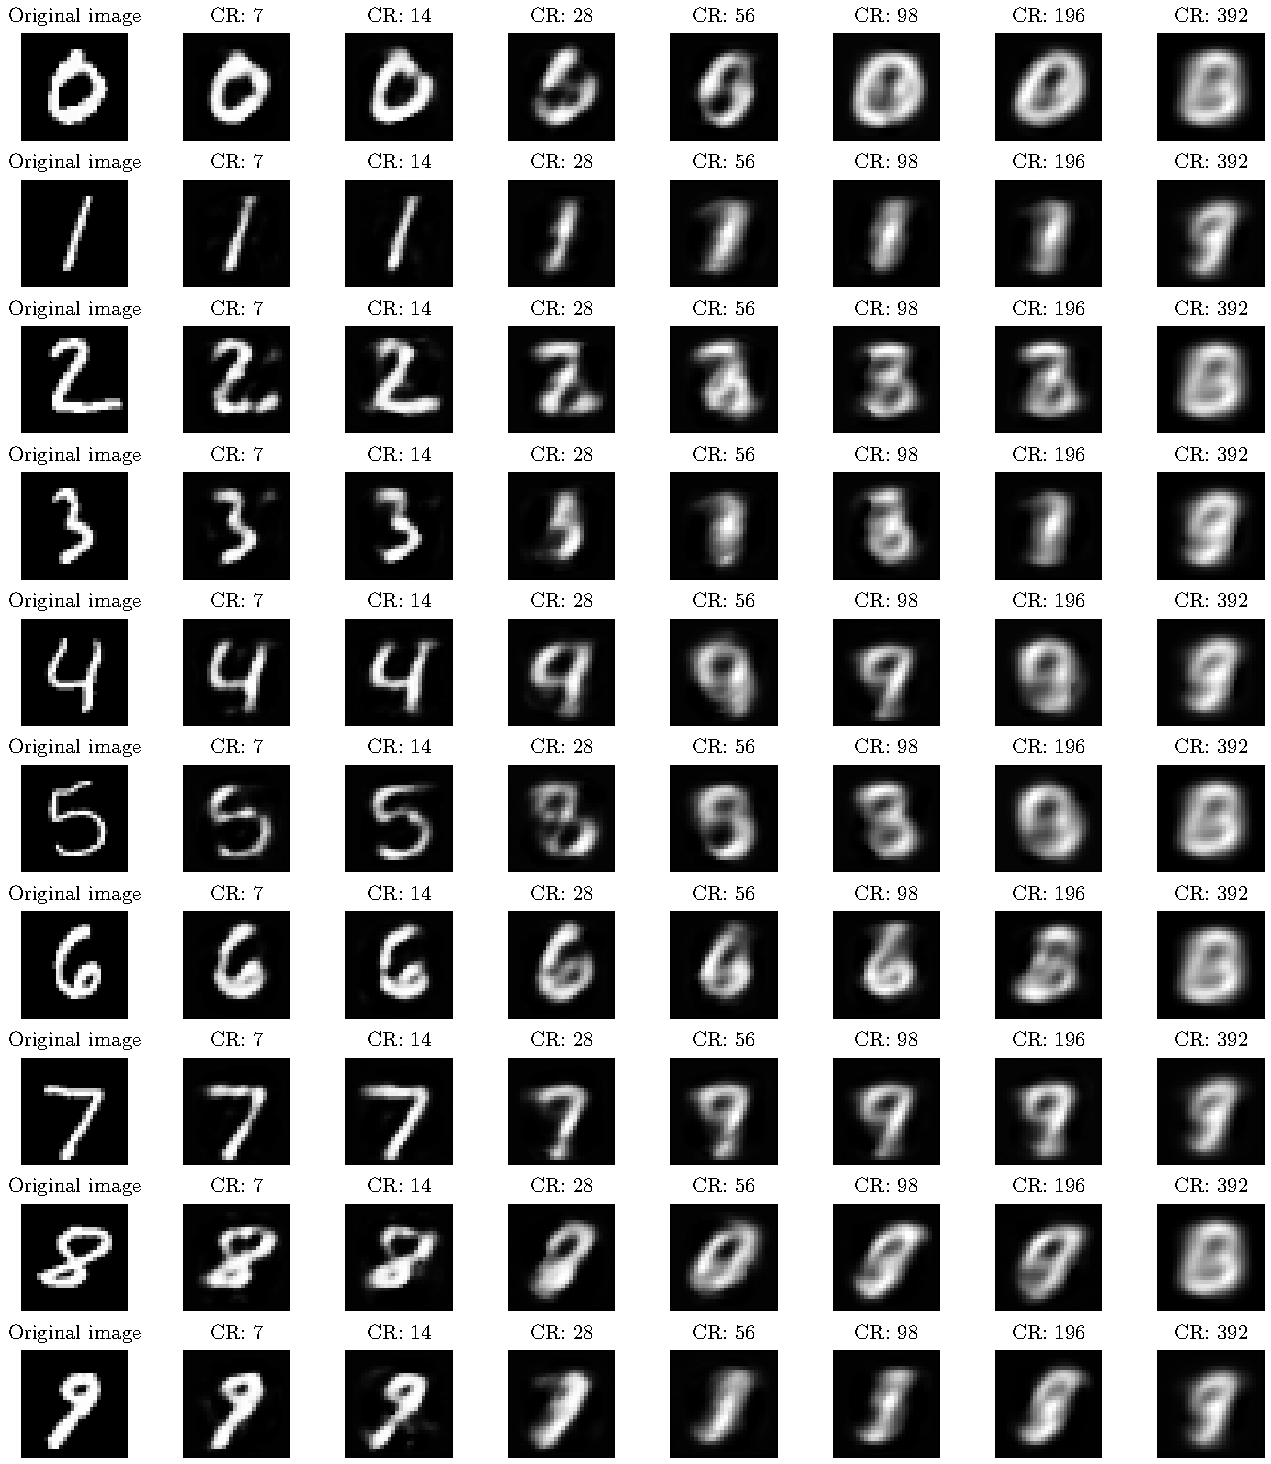
\includegraphics[width=1.0\textwidth]{graphics/decoded_instances.pdf}
    \textbf{Notes}: Reconstructed images are generated by encoding and decoding a stimulus image using a trained autoencoder networks with varying hidden layers, and bias set to zero. Columns separate reconstructed images by compression ratio (CR). Rows separate reconstructed images by the input stimulus (uncompressed) image. The first entry in each row is the stimulus image used to generate the following reconstructions.
\end{figure}

\begin{figure}
    \caption{Reconstructed instances disaggregated by compression ratio (including bias units)}
	\label{fig:decoded-instances}
	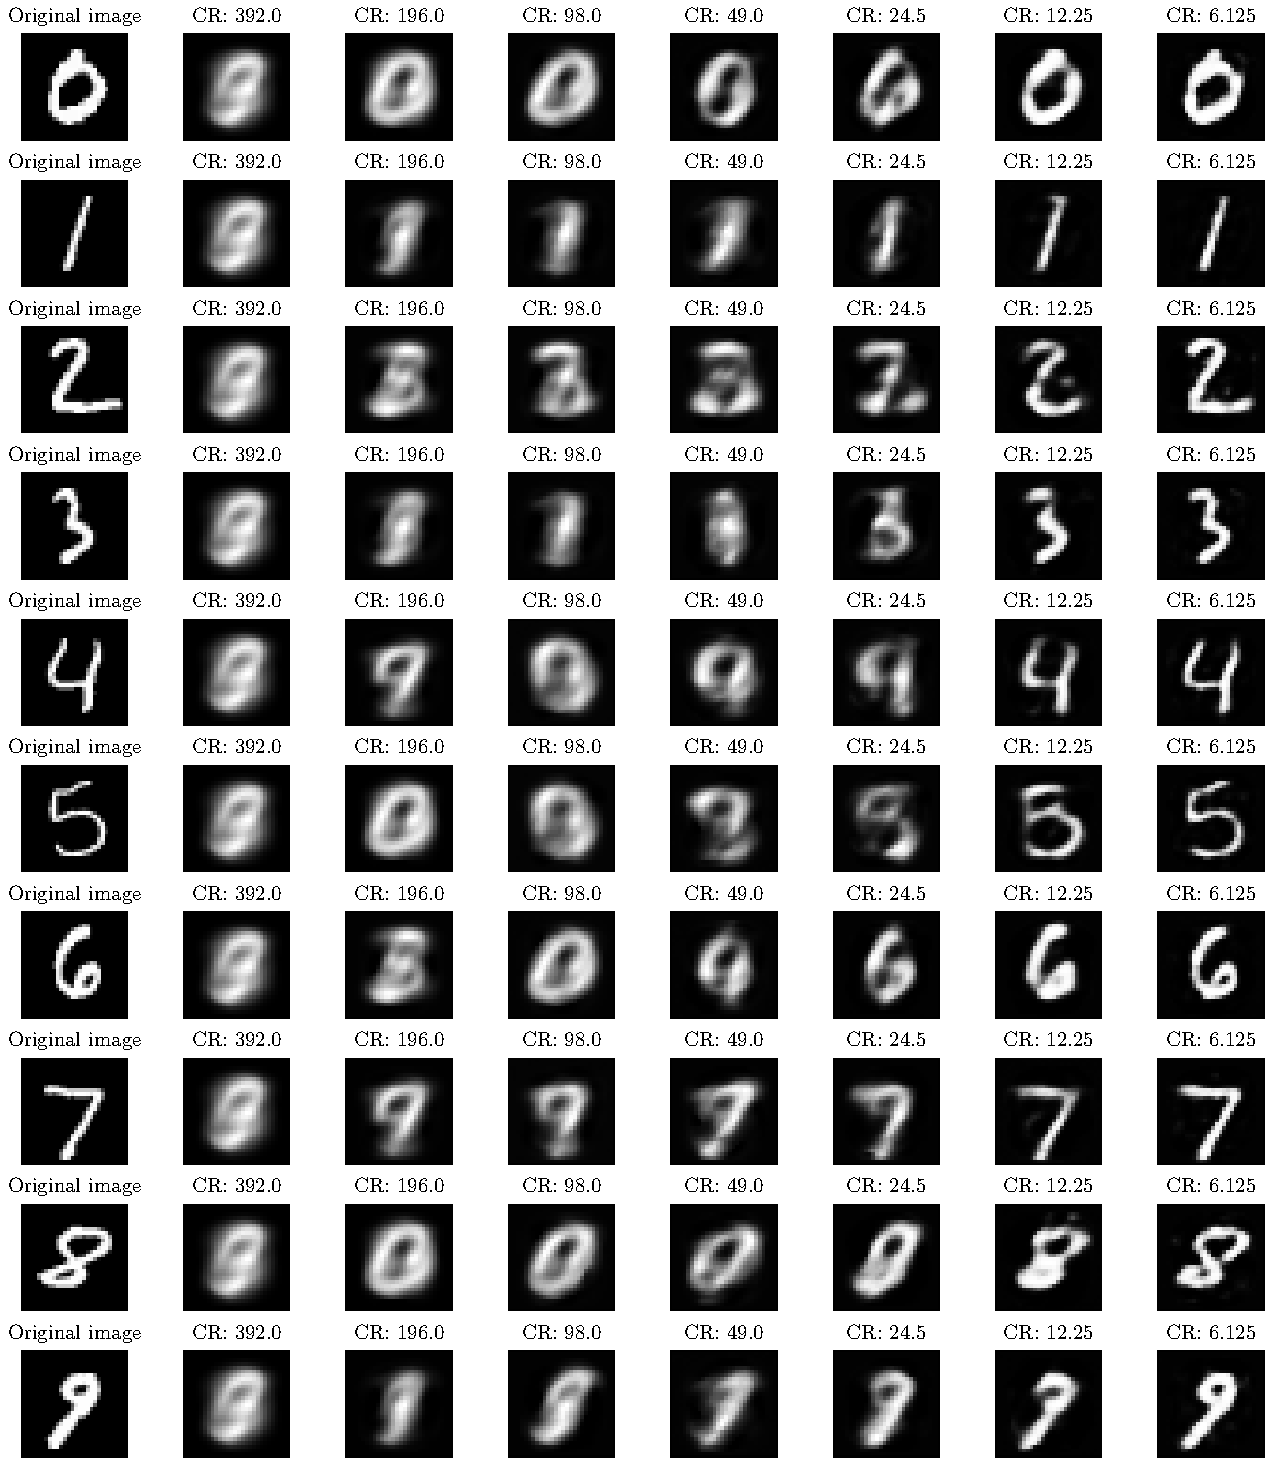
\includegraphics[width=1.0\textwidth]{graphics/decoded_instances_bias.pdf}
    \textbf{Notes}: Reconstructed images are generated by encoding and decoding a stimulus image using a trained autoencoder networks with varying hidden layers, and bias units included. Columns separate reconstructed images by compression ratio (CR). Rows separate reconstructed images by the input stimulus (uncompressed) image. The first entry in each row is the stimulus image used to generate the following reconstructions.
\end{figure}

\begin{figure}
    \caption{Mean-squared error (MSE) disaggregated by MNIST class}
	\label{fig:decoded-instances}
	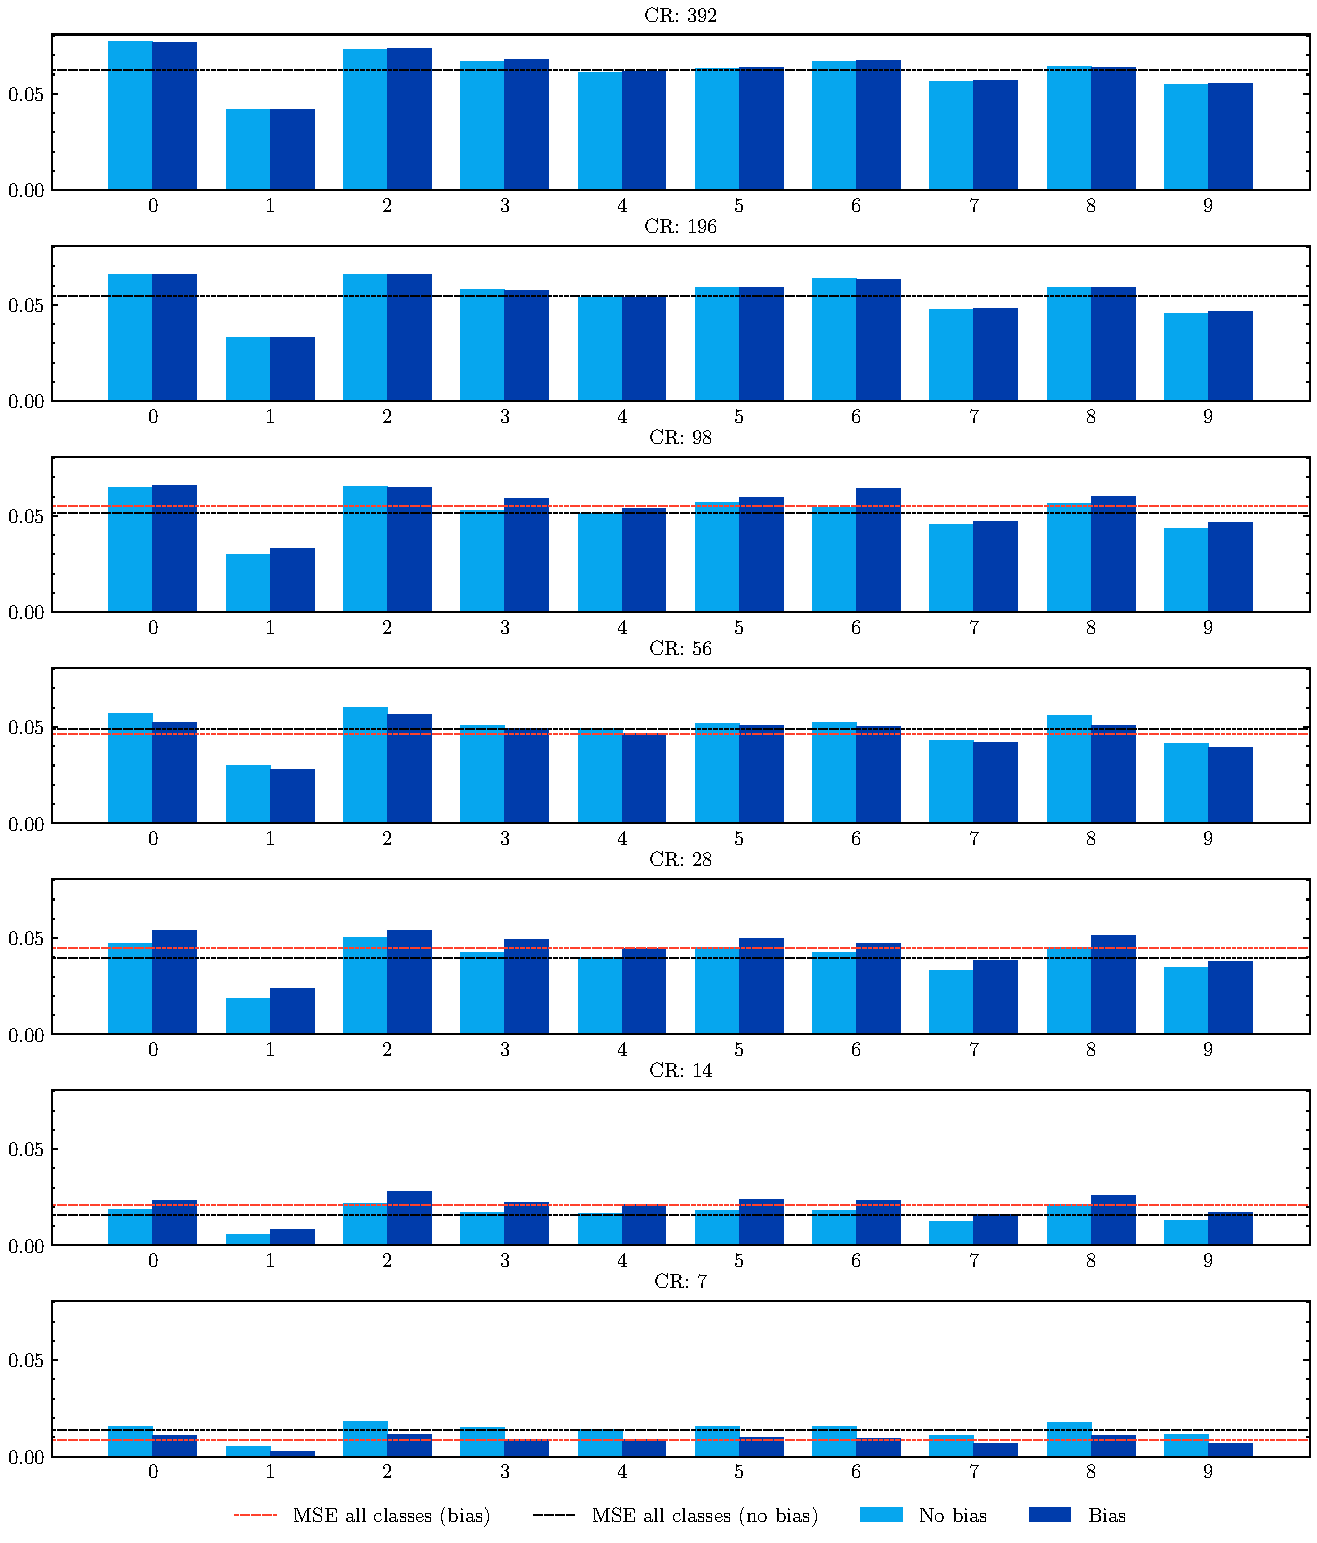
\includegraphics[width=1.0\textwidth]{graphics/mse_by_class.pdf}
    \textbf{Notes}: Mean squared error (MSE) across validation partition of MNIST dataset (N=10,000), disaggregated by annotated class of image instance. MSE is calculated after training models for 50 epochs. Autoencoder network architectures are split by compression ratio (CR), and inclusion of bias units.
\end{figure}


\begin{table}[h]
	\caption{Mean-squared error (MSE) for reconstructed images \label{table:mse-final}}
	\centering
	\begin{tabular}{lrrrr}
		\toprule
			Model &  MSE  \\
		\midrule
			\addlinespace{}
			\parbox{12.5cm}{Compression ratio: 392} & 0.0621 \\
			\addlinespace{}
			Compression ratio: 392 (bias) 	& 0.0624 \\
			\addlinespace{}
			Compression ratio: 196 			& 0.0547 \\
			\addlinespace{}
			Compression ratio: 196 (bias) 	& 0.0548 \\
			\addlinespace{}
			Compression ratio: 98 			& 0.0516 \\
			\addlinespace{}
			Compression ratio: 98 (bias) 	& 0.0551 \\
			\addlinespace{}
			Compression ratio: 56 			& 0.0488 \\
			\addlinespace{}
			Compression ratio: 56 (bias)	& 0.0463 \\
			\addlinespace{}
			Compression ratio: 28 			& 0.0395 \\
			\addlinespace{}
			Compression ratio: 28 (bias) 	& 0.0446 \\
			\addlinespace{}
			Compression ratio: 14 			& 0.0160 \\
			\addlinespace{}
			Compression ratio: 14 (bias) 	& 0.0208 \\
			\addlinespace{}
			Compression ratio: 7 			& 0.0138 \\
			\addlinespace{}
			Compression ratio: 7 (bias) 	& 0.0085 \\
	\bottomrule
	\addlinespace[1em]
	\end{tabular}
	\parbox{14.5cm}{\textbf{Notes}: Mean squared error (MSE) across validation partition of MNIST dataset (N=10,000) for reconstructed images. MSE is calculated after training models for 50 epochs.}
\end{table}

